\subsection{Zadanie 1}

Niech $(\Omega, F ,P)$ będzie przestrzenią probabilistyczną oraz niech \\ $A,B, A_1,A_2, \ldots, A_n \in F$. Pokazać że:\\ \\

\medskip
\noindent{\bf Podpunkt 1} 
\medskip

Prawdopodobieństwo zdarzenia niemożliwego jest równe zero
$$
P(\emptyset) = 0
$$

Wezmy przykladowa przestrzen $\Omega$ zawierajaca wszystkie mozliwe zdarzenia, ktore zachodza i wezmy przeciwstawne puste zdarzenie $\emptyset$ , ktore nigdy nie zachodzi.


$$ P(\Omega) = 1 \hspace{0.5cm} i \hspace{0.5cm}  P(\emptyset) = 0 $$

Dowod: \\

$$P(\Omega \cup \emptyset) = P(\Omega) + P(\emptyset)$$

Poniewaz $\Omega$ i $\emptyset$ sa wzajemnie sie wykluczajace zatem: 

$$ P(\emptyset) = 0 $$

\medskip
\noindent{\bf Podpunkt 2} 
\medskip


Skończona addytywność. Jeżeli $A_1,A_2, \ldots, A_n$ wykluczają się parami (tj, $A_i \cap A_j = 0$ dla $i \neq j$), to
$$
P\left(\bigcup_{i=1}^{n} A_i \right) = \sum_{i=1}^{n} P(A_i).
$$

$$\sum_{i=1}^{n} P(A_i) = P(A_1) + P(A_2) + \ldots + P(A_n)$$

Poniewaz sa one parami rozlaczne 

$$ P(A_i \cap A_j) = \emptyset , i \neq j$$

\medskip
\noindent{\bf Podpunkt 3} 
\medskip

$$
P(A') = 1 - P(A)
$$\\

Wezmy zdarzenia $A$ i $A'$ takie, ze $P(A \cup A') = \Omega$ i sa one rozlaczne.\\

Stad wiemy, ze:

$$P(A) + P(A') = P(A \cup A') = P(\Omega) = 1$$
Stad:
$$P(A') = 1 - P(A)$$


\medskip
\noindent{\bf Podpunkt 4} 
\medskip

Jeśli $A \subset B$, to 
$$
P(B \setminus A) \leq P(B) - P(A)
$$\\\\


Jesli $A \subset B$ to $ B = A \cup(B \setminus A) $ i $ A \cap (B \setminus A) = \emptyset $ \\
Stad:\\
$$ P(B) = P(A) + P(B \setminus A) $$ 
$$ P(B\setminus A) \geq 0 $$ 

Stad mamy, ze:

$$ P(B) \geq P(A) $$

\medskip
\noindent{\bf Podpunkt 5} 
\medskip

$$
P(A) \leq 1
$$

Zalozmy, ze $\Omega$ jest przestrzenia zawierajaca wszystkie zdarzenia A, wtedy:

$$ P(\Omega) = 1 $$

$$ P(A) \leq P(\Omega) = 1 $$

\medskip
\noindent{\bf Podpunkt 6} 
\medskip


$$
P(A \cup B) = P(A) + P(B) - P(A \cap B)
$$

Wynika z ponizszego diagramu. 

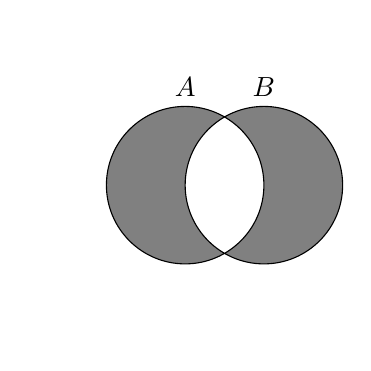
\begin{tikzpicture}[fill=gray]

% left hand
\scope
\clip (-2,-2) rectangle (2,2)
(1,0) circle (1);
\fill (0,0) circle (1);
\endscope
% right hand
\scope
\clip (-2,-2) rectangle (2,2)
(0,0) circle (1);
\fill (1,0) circle (1);
\endscope
% outline
\draw (0,0) circle (1) (0,1)  node [text=black,above] {$A$}
(1,0) circle (1) (1,1)  node [text=black,above] {$B$};

\end{tikzpicture}

